\chapter{FFT y su uso en las comunicaciones}

La Transformada Rápida de Fourier (Fast Fourier Transform o FFT por sus siglas
en inglés) es la denominación colectiva para un grupo de algoritmos que permiten
el cálculo eficiente de la Tranformada Discreta de Fourier (DFT) y posibilitan
su implementación en sistemas digitales a un costo menor que el cálculo de la DFT en forma
directa \cite{Schaffer2_1}. Cuando se habla de costo se refiere a caracerísticas mensurables de la
arquitectura como el tamaño, tiempo de ejecución, consumo, etc.

En este capítulo se presenta un resumen de las características de la
transformada de Fourier de tiempo continuo y de su versión discreta, y de la transformada rápida de
Fourier y su importancia en las comunicaciones digitales.

\section{La Transformada de Fourier}

La transformada de Fourier permite obtener la representación o descomposición en
el dominio de las frecuencias de señales representadas en el dominio del tiempo. Esta
representación permite un análisis más amplio de las señales y facilita el estudio de 
los efectos de los sistemas sobre las mismas y el procesamiento de señales
en general.

No es la intención de este trabajo extenderse en la teoría de la Transformada de
Fourier por lo que se omiten los cálculos referentes a la deducción de las
ecuaciones correspondientes a las diferentes formas de la misma. Estas deducciones se pueden
encontrar en \cite{Schaffer2_2}\cite{Meyer2_1}.
 
\subsection{Transformada de Fourier de tiempo continuo}

La descomposición en series de Fourier de señales periódicas permite descomponer señales con período
finito en el tiempo en una suma de exponenciales complejas equiespaciadas que representan los
armónicos en frecuencia que componen la señal. Teniendo en cuenta la utilidad que tiene esta
representación en el análisis y procesamiento de señales periódicas (análisis de sistemas LTI,
diseño de filtros, etc.) resulta de interés poder analizar de la misma manera señales no periódicas.

Pensando una señal de duración finita $x(t)$ como un ciclo de una señal
periódica $\tilde{x}(t)$ se puede plantear la representación en serie de
Fourier de la misma \cite{Schaffer2_3}. Una vez expresada la sumatoria que describe la serie de
Fourier se puede tomar su límite cuando el período tiende a
infinito (ya que se puede pensar una señal aperiódica como una señal periódica
de período infinito) convirtiendo la sumatoria en una integral. A
través de una deducción matemática \cite{Schaffer2_3} se llega al siguiente par de ecuaciones:

\begin{equation}
X(j\omega) = \int_{-\infty}^{\infty}x(t)e^{-j\omega t}d\omega
\label{eq:TF}
\end{equation}

\begin{equation}
x(t) = \frac{1}{2\pi}\int_{-\infty}^{\infty}X(j\omega)e^{j\omega t}d\omega
\label{eq:iTF}
\end{equation}


(\ref{eq:TF}) y (\ref{eq:iTF}) son conocidas como el par de
transformadas de Fourier, cuya función $X(j\omega)$ es la \emph{Transformada de
Fourier} de la señal $x(t)$ y (\ref{eq:iTF}) es la ecuación de
la \emph{transformada inversa de Fourier}.

\subsection{Transformada de Fourier en Tiempo Discreto}

La transformada de Fourier en tiempo continuo es una gran herramienta
para el análisis de señales, pero la imposibilidad de procesar la transformada de Fourier para
señales reales sumado al gran costo computacional de la aproximación numérica utlizando punto
flotante lleva a la búsqueda de una alternativa que posibilite el procesamiento digital. Esto se ve
potenciado además por el avance de los procesadores digitales, tanto en velocidad como en capacidad
de cómputo, costo, etc. Teniendo en cuenta todo esto y para aprovechar el potencial del
procesamiento digital se llega a la Transformada de Fourier en Tiempo Discreto (DFT, Discrete Fourier Transform)
donde se utilizan N muestras tanto en tiempo como en frecuencia \cite{Schaffer2_3}.
Además, como se describe en la sección \ref{sec:dftOfft}, existen algoritmos eficientes para su
cómputo lo que posibilita su implementación práctica en sistemas digitales.

Tomando como base la descompocisión en series de Fourier de una secuencia
periódica y su transformada de Fourier a través de sus coeficientes se
llega a las ecuaciones que definen la Transformada de Fourier en Tiempo
Discreto a través de un razonamiento similar al de la transformada continua de
Fourier tomando una secuencia finita $x[n]$ de longitud N como un período de una
secuencia $\tilde{x}[n]$ de período N:

\begin{equation}
X[k] = \sum_{n=0}^{N-1}x[n]W_N^{kn}
\label{eq:DTF}
\end{equation}

\begin{equation}
x[n] = \frac{1}{N}\sum_{k=0}^{N-1}X[k]W_N^{-kn}
\label{eq:iDTF}
\end{equation}

donde $W_N^{kn}=e^{\frac{-j2\pi kn}{N}}$, comunmente llamdos \textit{twiddle factors}.

(\ref{eq:DTF}) es la ecuación de la DFT mientras que (\ref{eq:iDTF}) es la ecuación de la
transformada inversa de Fourier en Tiempo Discreto (IDFT) también conocida como ecuación de síntesis. Esta última
ecuación muestra como la señal $x[n]$ se representa como una combinación lineal
de exponenciales complejas o desde otro punto de vista como una combinación
lineal de componentes en frecuencia.

Como ejemplo se ve en la figura \ref{fig:escalon_16} un pulso rectangular continuo de
longitud $8$ y su versión muestreada con $N=16$. Este pulso se puede tomar como un ciclo de una
onda cuadrada de período $16$.
En la figura \ref{fig:fourier_escalon} se presenta la transformada continua de
Fourier y la transformada en tiempo discreto de Fourier en color azul y rojo
respectivamente. Se aprecia como la DFT es un muestreo de la transformada
continua, con $N=16$, equiespaciado en frecuencia.

\begin{figure}[htb!]
        \centering
        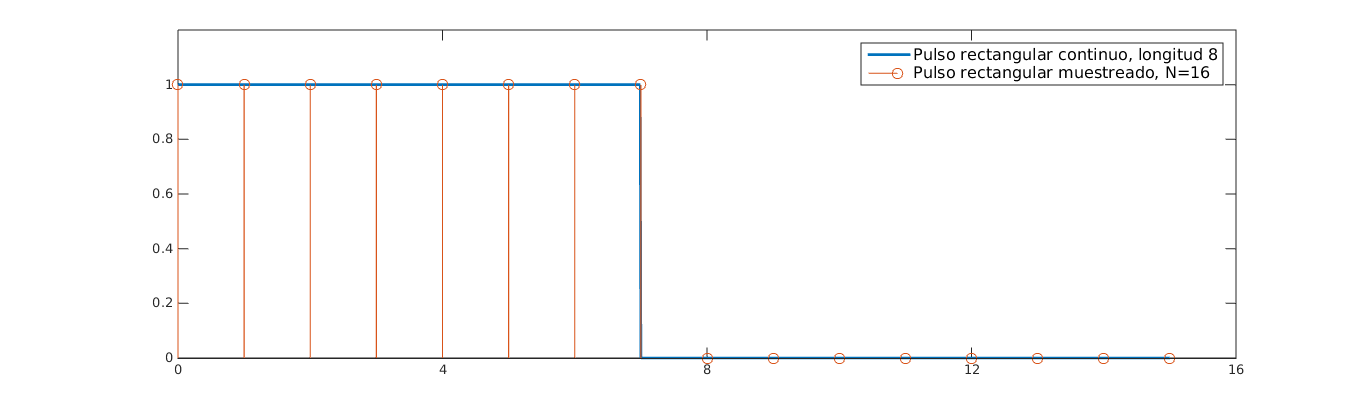
\includegraphics[width=12cm]{./figures/pulso_rect.png}
        \caption{Pulso rectangular de longitud 8, continuo y muestreado con N=16}
        \label{fig:escalon_16}
\end{figure}

\begin{figure}[htb!]
        \centering
        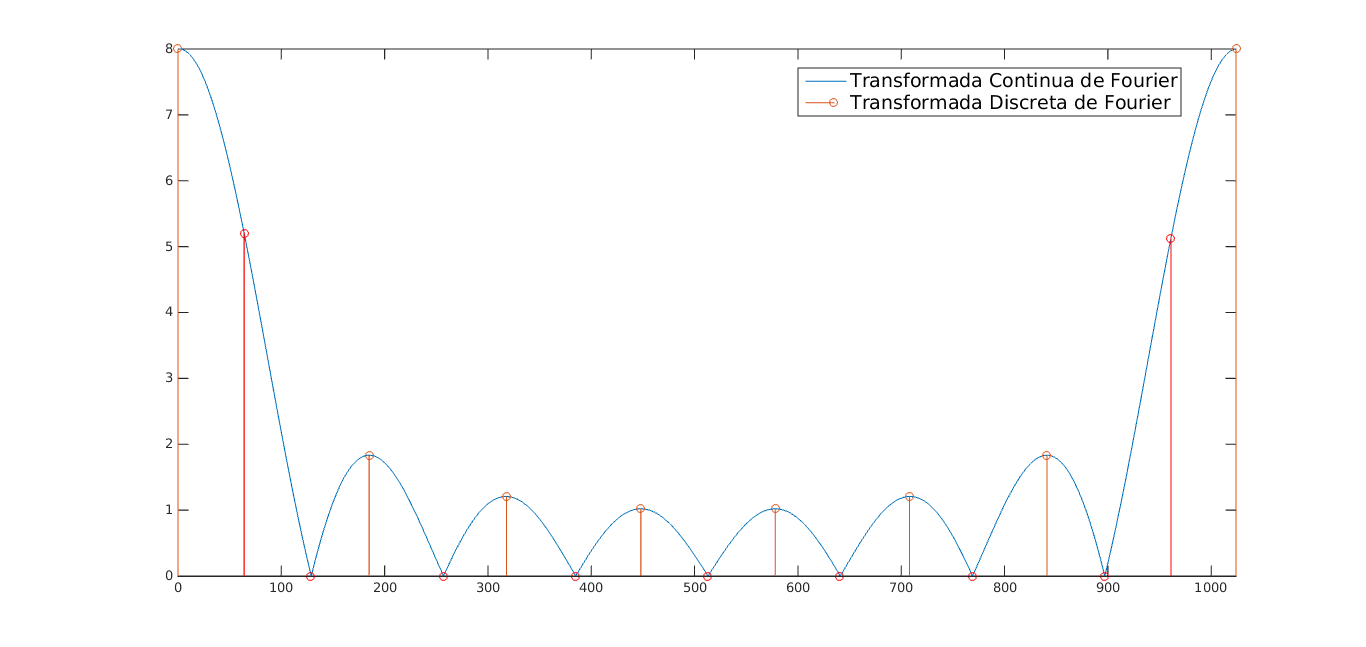
\includegraphics[width=12cm]{./figures/FT_DFT.png}
        \caption{Transformada de Fourier de un pulso rectangular}
        \label{fig:fourier_escalon}
\end{figure}

Se debe recordar los efectos del muestreo en tiempo y en frecuencia:
\begin{itemize}
  \item Al muestrear en tiempo se obtiene un espectro periódico con frecuencia
  de muestreo $f_s$. La aproximación de la transformada de Fourier a través
  de la DFT es razonable si las componentes en frecuencia de $x(t)$ están
  concentradas en un rango menor a la frecuencia de Nyquist $f_s/2$ de acuerdo con el
  teorema de muestreo de Shannon \cite{Shannon}.
  \item Al muestrear en frecuencia la función temporal se vuelve periódica, esto
  es, la DFT asume a la función $x(t)$ como periódica. Por este motivo se debe
  utilizar una frecuencia de muestreo y una ventana de análisis de forma que
  cubran un número entero de períodos de $x(t)$ (o períodos teóricos en caso
  que $x(t)$ no sea periódica) en N muestras para evitar anomalías en la
  transformada, tales como leakage, ripple, etc.
\end{itemize}

\section{La Transformada Rápida de Fourier} \label{sec:fft}

La implementación directa de la DFT según (\ref{eq:DTF}) implica que
para cada una de las N salidas del cálculo se requieren N operaciones
aritméticas, N sumas, lo que equivale a una complejidad del orden de
$\Theta(N^2)$, lo cual es inaceptables en sistemas escalables. Por esto históricamente se buscaron
formas más eficientes de realizar el cálculo de la DFT. Estos algoritmos se conocen globalmente como Tranformada Rápida de
Fourier (FFT, Fast Fourier Transform), que permiten reducir la
complejidad al orden de $\Theta(N*\log(N))$ \cite{Schaffer2_2}\cite{Schaffer2_1}.

Los algoritmos de FFT utilizan la estrategia \emph{divide y vencerás} a través de
una transformación de una DFT de longitud N (\ref{eq:DTF}) en una
representación multidimensional $N=\Pi_lN_l$. Esto permite dividir el cálculo de
una DFT de $N$ puntos en múltiples DFT de $N_l$ reduciendo de esta manera la
complejidad computacional total.

Como ejemplo se analizará brevemente la descompocisión en dos dimensiones.
Se transforma el índice temporal $n$ según

 \begin{equation}
n = An_1 + Bn_2 \ mod\ N \qquad 
	\begin{cases}
	0\leq n_1 \leq N_1 -1 \\
	0\leq n_2 \leq N_2 -1
	\end{cases}
\label{eq:timeInedx}
\end{equation}

Donde $N=N_1*N_2$ y $A,B \in Z$ son constantes a definir. Usando esta
transformación se construye un mapeo bidimensional del tipo $f:C^N\rightarrow
C^{N_1xN_2}$.

Aplicando una transformación similar al índice k en el dominio de la frecuencia:

\begin{equation}
k = Ck_1 + Dk_2 \ mod\ N \qquad 
	\begin{cases}
	0\leq k_1 \leq N_1 -1 \\
	0\leq k_2 \leq N_2 -1
	\end{cases}
\label{eq:freqInedx}
\end{equation}

Donde $C,D \in Z$ son constantes a definir. Como la DFT es biyectiva se debe
tener precaución en la elección de los coeficientes A, B, C y D para que la
nueva representación de la transformada siga teniendo esta característica.

Esta representación implica la separación de la DFT de $N$ puntos en dos DFT de
$N_1$ y $N_2$ puntos aplicadas una a continuación de la otra. Esta
representación se puede realizar de forma recursiva y subdividir a su vez $N_1$
como $N_1 = N_{11}N_{12}$ y así sucesivamente.

Los algoritmos de FFT permiten un cálculo eficiente de la DFT no solo en tiempo
de cálculo sino también en complejidad de código en caso de software y en
complejidad, tamaño y consumo en caso de hardware haciendo posible su implementación
en circuitos integrados.

Los diferentes algoritmos de FFT se diferencian entre sí por los valores
que asignan a los coeficientes $A,\ B,\ C\ y\ D$. Existen algoritmos que
permiten aprovechar esta optimización del cálculo dependiendo de la naturaleza
de la señal y el objetivo del cálculo para cualquier longitud de la DFT.

\section{Uso de la DFT en las comunicaciones digitales}
\subsection{Multiplexación por división ortogonal de frecuencia (OFDM)}

La creciente demanda de servicios de comunicación inalámbrica lleva a la
necesidad de aumentar el flujo de datos transmitidos a través de
radiofrecuencias. Tratar de llevar la velocidad de transmisión de símbolos para
alcanzar tasas de bits del orden del Mbit o mayores requiere la utilización de
ecualización adaptativa lo que eleva la complejidad y el costo de los equipos
utilizados \cite{Prasad2_1}.
Una forma de encarar el problema es la multiplexación en frecuencia, donde los
símbolos en los que se modula la información se multiplexan en múltiples
portadoras y se transmiten en forma simultánea aumentando de esta forma la tasa de transferencia de
bits sin necesidad de aumentar la frecuencia o la complejidad de los símbolos utilizados en la
modulación. Otra ventaja de la transmisión multiportadora es su robustez frente a interferencia selectiva en frecuencia ya
que solo se verían afectadas algunas de las portadoras y el error provocado se
puede corregir mediante un sistema de corrección de errores. 

En los sistemas tradicionales de transmisión multiportadora la banda de
frecuencia total se divide en $N$ canales sin superposición los cuales son
modulados por diferentes símbolos y multiplexados en frecuencia. La transmisión simultánea de
múltiples frecuencias presenta el riesgo de interferencia entre portadoras (ICI, Inter Charrier
Interference) por lo que los canales deben separarse de forma de reducir la interferencia entre
ellos, lo que lleva a un aprovechamiento ineficiente del espectro disponible.
Para mejorar la eficiencia en el uso del ancho de banda a mediados de la
década de 1960 se propuso la utilización de transmisión en paralelo, al igual
que en el sistema tradicional, y la multiplexación en frecuencia sobre canales
superpuestos, que llevando una velocidad de símbolo $b$ son espaciados entre si una
distancia $b$ en frecuencia para disminuir el ruido impulsivo y distorsión por
caminos múltiples además de aprovechar mejor el ancho de banda \cite{Prasad2_1}.                  
En la figura \ref{fig:portadoras} se ve la diferencia en el aprovechamiento 
del ancho de banda al transmitir $8$ subportadoras separadas y las mismas $8$ 
subportadoras superpuestas.

\begin{figure}[htb!]
        \centering
        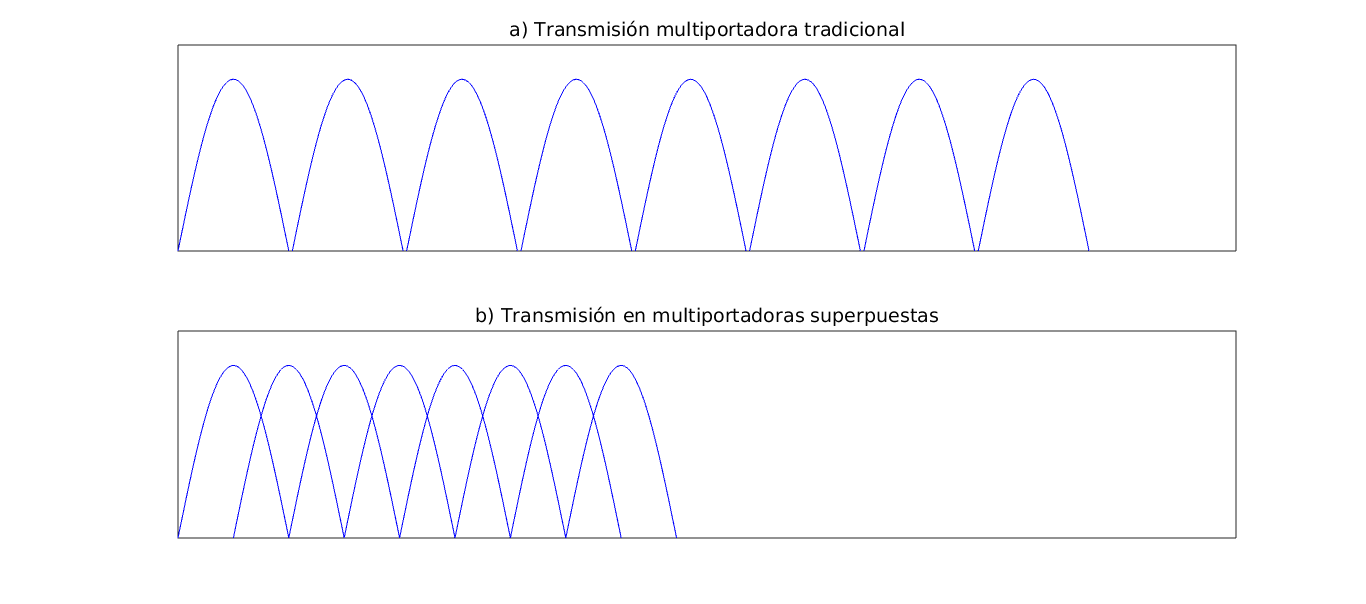
\includegraphics[width=17cm]{./figures/trad_mult.png}
        \caption{Dos formas de transmisión multiportadora}
        \label{fig:portadoras}
\end{figure}

El sistema de multiplexado en división de frecuencias ortogonales (OFDM, 
Orthogonal Frecuency-Division Multiplexing) propone la utilización de
frecuencias  matemáticamente ortogonales para reducir la interferencia entre las
portadoras. Con el receptor actuando como un banco de demoduladores
que traslada cada subportadora a banda base, se realiza una integración sobre un
período de la señal de esa subportadora para recuperar la información. Si las demás
portadoras tienen un número entero de ciclos durante ese período ($T$), luego de la
integración la contribución de estas a la subportadora que se está procesando es nula. Entonces las
portadoras serán ortogonales si están separadas un múltiplo de $1/T$. La figura \ref{fig:OFDM_ports} 
muestra un conjunto de subportadoras conformando una señal OFDM.

\begin{figure}[htb!]
        \centering
        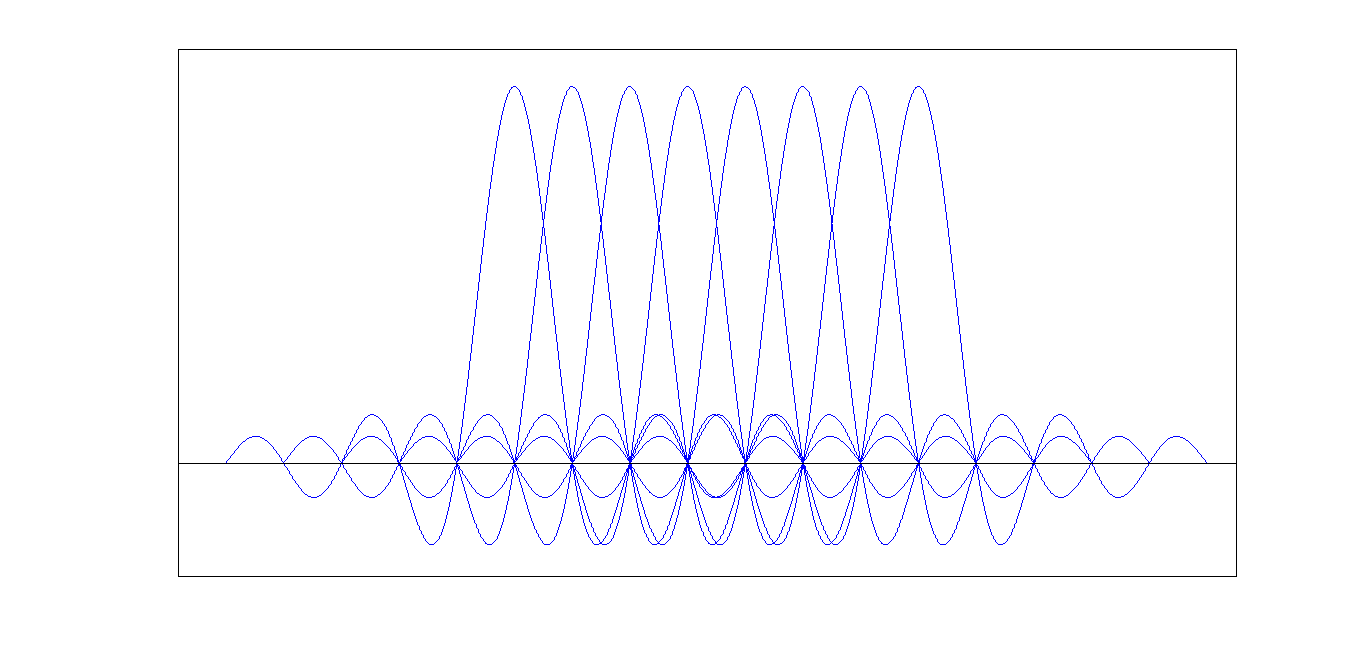
\includegraphics[width=17cm]{./figures/ofdm_subcarriers.png}
        \caption{Idea conceptual de una señal OFDM}
        \label{fig:OFDM_ports}
\end{figure}

El sistema de transmisión por OFDM se utiliza en muchos tipos de
comunicación actuales siendo uno de los sistemas más extendidos \cite{Prasad2_1}. Este sistema
está presente en las conexiones de datos tipo DSL, en las redes inalámbricas
(WLAN, WPAN) de tipo Wi-Fi, WiMax, etc, en las transmisiones de video y audio
digital (DAB/DVB) entre otros muchos medios de transmisión de información.

Si bien por si sola la modulación OFDM presenta varias ventajas en la
transmisión de datos esto no alcanza para una implementación práctica ya que
deben tenerse en cuenta las características distorisivas del canal.

Una de las modificaciones principales sobre el sistema teórico es el agregado de
un intervalo de guarda (GI sus siglas en inglés) utilizado para reducir el
efecto del delay producido por la característica multi-camino del canal. Este
GI está compuesto por la repetición de la porción final del símbolo transmitido
al principio del mismo, convirtiendo el símbolo en periódico. Esta porción
agregada se conoce como prefijo cíclico. Gracias al prefijo cíclico el efecto
dispersivo en tiempo del canal se reduce a una convolución cíclica por lo que
con solo descartar el GI en el receptor se obtiene el símbolo completo.
Además, gracias a las características de la convolución cíclica o circular, se
preserva la ortogonalidad de las subportadoras. La desventaja de aplicar el
prefijo cíclico es la disminución en la eficiencia del uso del ancho de banda
al agregar información no útil a la transmisión. La duración del GI
($T_{guard}$) es seleccionada para que sea mayor al máximo delay del canal. Por
lo tanto la parte efectiva de la señal recibida puede ser vista como la
convolución cíclica del símbolo transmitido por la respuesta impulsiva del
canal.

Por otro lado un pulso rectangular tiene un gran ancho de banda debido a los
lóbulos laterales de la sinc que compone su espectro. Para reducir la potencia
transmitida fuera del ancho de banda del símbolo se agrega un tiempo de ventana
a la transmisión con una forma de onda que cae progresivamente, a diferencia del
pulso rectangular, lo que reduce los lóbulos lateralesde la sinc reduciendo a su
vez el ancho de banda total del símbolo. Esta ventana se agrega al inervalo de
guarda descipto anteriormente aumentando la robustez respecto de la
dispersividad del canal pero reduciendo aún más la eficiencia ya que esta
ventana también es descartada por el receptor.

\begin{figure}[htb!]
        \centering
        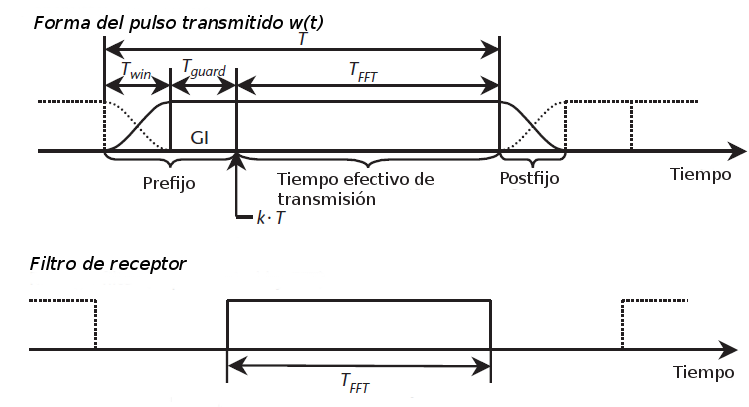
\includegraphics[width=12cm]{./figures/symbol_T.png}
        \caption{Diagrama de tiempos de un símbolo OFDM}
        \label{fig:symbol_T}
\end{figure}

Esto queda ejemplificado en la figura \ref{fig:symbol_T} donde se ve el esquema
de tiempos de un símbolo OFDM. Como este procesamiento se realiza habitualmente en
hardware digital estos tiempos suelen expresarse en muestras. $T$ ($N$),
$T_{FFT}$ ($N_{FFT}$), $T_{guard}$ ($N_{guard}$) y $T_{win}$ ($N_{win}$)
representan los tiempos (número de muestras) del símbolo transmitido, su parte
efectiva, el GI y el tiempo de ventana respectivamente.

En la figura \ref{fig:OFDM_blocks} se
observa un diagrama en bloques de un transmisor OFDM. La data de origen es dividida en paquetes/canales y mapeada a lo símbolos
respectivos de la constelación correspondiente a la modulación seleccionada para la transmisión.
Esos símbolos, que componen una constelación de símbolos complejos, es modulada en las
multiportadoras ortogonales para su transmisión y se le agrega el intervalo de guarda para luego
convertir la señal resultante digital en una señal analógica para ser transmitida. Una vez recibida
esta señal en el receptor, es digitalizada para su procesamiento y se remueve el intervalo de
guarda. La porción de información efectiva de la señal es enviada al demodulador OFDM que extrae la
constelación de puntos complejos que es demapeada en la información original.
El presente trabajo se enfoca en desarrollar los bloques de modulación y demodulación OFDM del
diagrama de bloques expuesto.


\begin{figure}[htb!]
        \centering
        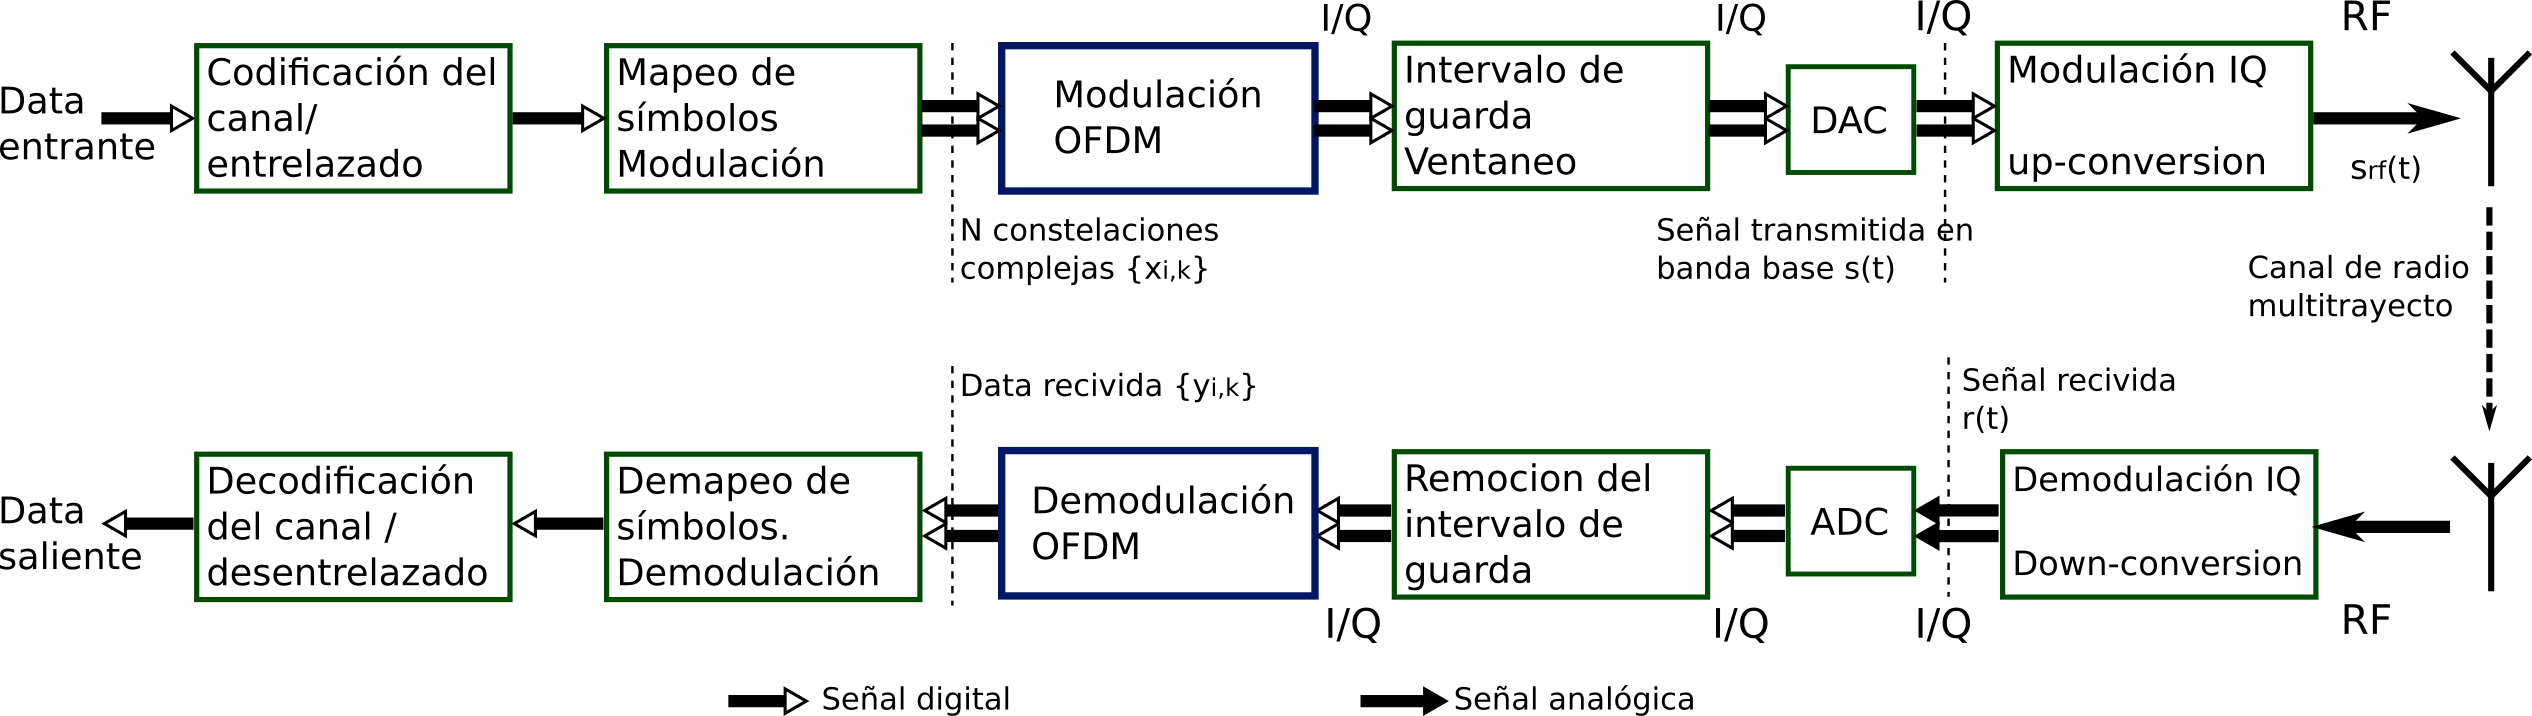
\includegraphics[width=15cm]{./figures/ofdm_blocks.png}	%OFDM_block_1
        \caption{Diagrama en bloques de una transmisión punto a punto OFDM}
        \label{fig:OFDM_blocks}
\end{figure}

\subsection{Implementación de la modulación OFDM mediante DFT}

Matemáticamente la OFDM se expresa como la suma de los pulsos base desplazados
en tiempo y frecuencia y multiplicados por los símbolos de datos.
En notación temporal, el k-ésimo símbolo de una señal OFDM se escribe como:

\begin{equation}
s_{RF,k}(t-kT) = 
%	\begin{cases}
	Re\left\{ w(t-kT) \sum\limits_{i=-N/2}^{N/2-1} x_{i,k} e^{j2\pi
	\left(f_c+\frac{i}{T_{FFT}}\right)(t-kT)}\right\}\\
%	\end{cases}
\label{eq:OFDM_symbol}
\end{equation}

para $kT-T\text{win}-T\text{guard}\leq t \leq kT+T_{FFT}+T\text{win}$ y $0$ para todo otro caso.

Donde:

\begin{itemize}
\item $T$: Duración de símbolo, tiempo entre dos símbolos consecutivos
\item $T_{FFT}$: Parte efectiva de un símbolo
\item $Tguard$: GI, duración del prefijo cíclico
\item $Twin$: intervalo de ventana
\item $k$: Índice del símbolo transmitido
\item $i$: Índice de subportadora, $i \in \{$$–N/2,\; –N/2+1,\; … –1,\; 0,\; 1,\; …
N/2–1$$\}$;
\item $x_{i,k}$: Punto de la constelación de la señal. Símbolo complejo
modulado en la i-ésima portadora del k-ésimo símbolo OFDM
\item $w(t)$: El pulso formador
\end{itemize}

Finalmente una secuencia continua de símbolos OFDM se expresa como:

\begin{equation}
s_{RF}(t) = \sum_{k=-\infty}^{\infty}s_{RF,k}(t-kT)
\label{eq:OFDM_seq}
\end{equation}

De estas ecuaciones se deduce la señal compleja equivalente en banda base:

\begin{equation}
s(t) = \sum_{k=-\infty}^{\infty}s_{k}(t-kT)
\label{eq:OFDM_low}
\end{equation}

donde

\begin{equation}
s_{k}(t-kT) =
%	\begin{cases}
	w(t-kT) \sum\limits_{i=-N/2}^{N/2-1} x_{i,k} e^{j2\pi
	\left(\frac{i}{T_{FFT}}\right)(t-kT)}
%	\end{cases}
\label{eq:OFDM_symbol_low}
\end{equation}

para $kT-T\text{win}-T\text{guard}\leq t \leq kT+T_{FFT}+T\text{win}$ y $0$ para todo otro caso. 

Se puede notar la similitud entre (\ref{eq:OFDM_symbol_low}) y 
(\ref{eq:iDTF}) de la IDFT donde $k$ representa la subportadora. Esta
similitud es sumamente importante ya que permite reemplazar los moduladores del
transmisor por el cálculo de una IDFT, o su versión de mayor eficiencia IFFT, y
el banco de filtros para demodular en el receptor por el cálculo de una DFT al realizar
procesamiento digital.
Esto representa una simplificación considerable en el diseño de sistemas OFDM y
su procesamiento mediante hardware digital o incluso por software  y ha motivado
el creciente estudio sobre la transformada discreta de Fourier y los algoritmos
de cálculo eficiente de la misma, buscando arquitecturas de procesamientos más eficiente, más
pequeñas, con menor consumo de energía/recursos, etc.

